% --------------------------------------------------------------
\begin{frame}[fragile]
  \frametitle{Separation Matrix Facility}
Separation needs to be elemental and should take an arbitrary incoming stream 
that is separated into streams based on a matrix of efficiencies. It should 
have input parameters:

\begin{itemize}
\item incoming commodity
\item outgoing commodities
\item map of element, stream, efficiency
\end{itemize}
\begin{figure}[htbp!]
\begin{center}
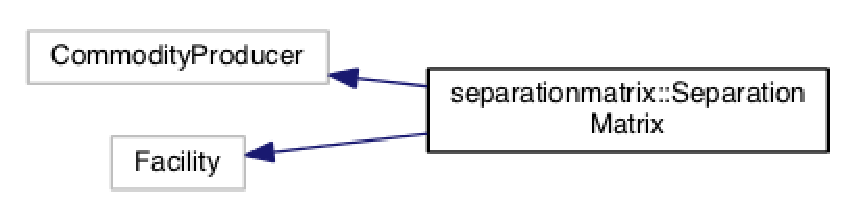
\includegraphics[width=0.8\textwidth]{sm_inherit}
\end{center}
\caption{Utilizes interfaces defined in Cyclus.}
\label{fig:sm_inherit}
\end{figure}
\end{frame}
% --------------------------------------------------------------
\begin{frame}[fragile]
  \frametitle{Separation Matrix Facility}
The efficiencies must be defined to transform :
\begin{itemize}
 \item an incoming composition vector, $I$, 
 \item with $N$ constituent amounts, 
 \item $I_n$ 
\end{itemize}
to 
\begin{itemize}
\item an outgoing set of $M$ streams,
\item $E_m$.
\end{itemize}

\end{frame}
% --------------------------------------------------------------
\begin{frame}[fragile]
The efficiency matrix, $\eta$, is therefore an $N\times M$ matrix of
efficiencies. The matrix of separation efficiencies has a default value: the
identity matrix of size $N\times N$. In this context, the identity matrix
represents complete and perfect elemental separation without losses. 
\begin{align*}
  \left[
    \begin{array}{c c c c c c c}
      \eta_{11} & . & . & . & . & . & \eta_{1M} \\
      \eta_{21} & . & . & . & . & . & \eta_{2M} \\
      . & . & . & . & . & . & . \\
      . & . & . & . & . & . & . \\
      . & . & . & . & . & . & . \\
      \eta_{N1} & .  & . & . & . & . & \eta_{NM} \\
    \end{array}
    \right]
  \left[
    \begin{array}{c}
      I_1\\
      I_2\\
      . \\
      . \\
      . \\
      I_N\\
    \end{array}
    \right]
    =
    \left[
      \begin{array}{ c }
        E_1\\
        E_2\\
        .\\
        .\\
        .\\
        E_M\\
      \end{array}
      \right]
\end{align*}
\end{frame}

% --------------------------------------------------------------
\begin{frame}[fragile]
\footnotesize{
\begin{lstlisting}
      <SeparationMatrix>
        <in_commod>sfr_unf_cool</in_commod>
        <out_commods>
          <val>rep_sfr_tru</val>
          <val>rep_sfr_u</val>
        </out_commods>
        <elems>
          <val>92</val>
          <val>94</val>
          <val>95</val>
        </elems>
        <effs>
          <val>1</val>
          <val>1</val>
          <val>1</val>
        </effs>
        <streams>
          <val>rep_sfr_u</val>
          <val>rep_sfr_tru</val>
          <val>rep_sfr_tru</val>
        </streams>
        <process_time>0</process_time>
      </SeparationMatrix>
  \end{lstlisting}
}
\end{frame}
